\documentclass[tikz,border=1mm]{standalone}
% Shared publication styles; labels designed for 170 mm inclusion width.
\usepackage[T1]{fontenc}
\usepackage{lmodern}
\usepackage{amsmath}
\usepackage{tikz}
\usepackage{pgfplots}
\pgfplotsset{compat=1.18}
\usetikzlibrary{arrows.meta,positioning,calc,fit,backgrounds,shapes.geometric,patterns,decorations.pathreplacing,circuits.logic.US}
\definecolor{ink}{HTML}{263238}
\definecolor{muted}{HTML}{60717D}
\definecolor{grid}{HTML}{DCE5EA}
\definecolor{normal}{HTML}{4C78A8}
\definecolor{compact}{HTML}{59A14F}
\definecolor{june}{HTML}{8A6BBE}
\definecolor{warn}{HTML}{C18523}
\definecolor{bad}{HTML}{BC514C}
\definecolor{phasezero}{HTML}{DBEAF8}
\definecolor{phaseone}{HTML}{DFEFD9}
\definecolor{phasetwo}{HTML}{FFF1C8}
\definecolor{phasethree}{HTML}{ECE1F6}
\tikzset{
  every picture/.style={font=\sffamily\fontsize{8}{9.5}\selectfont,text=ink},
  >=Latex,
  box/.style={draw=ink!60,fill=white,rounded corners=1.2pt,align=center,inner sep=4pt,line width=.55pt},
  flow/.style={-{Latex[length=1.7mm,width=1.2mm]},draw=ink,line width=.65pt},
  control/.style={flow,dashed,draw=muted},
  retry/.style={flow,draw=warn},
  paneltitle/.style={font=\sffamily\bfseries\fontsize{9}{10.5}\selectfont,anchor=west},
  smallnote/.style={font=\sffamily\fontsize{7}{8.5}\selectfont,text=muted,align=left},
  gridline/.style={draw=grid,line width=.2pt},
}
\pgfplotsset{every axis/.append style={
  font=\sffamily\fontsize{8}{9.5}\selectfont,
  label style={font=\sffamily\fontsize{8}{9.5}\selectfont},
  tick label style={font=\sffamily\fontsize{7.5}{9}\selectfont},
  legend style={font=\sffamily\fontsize{7.5}{9}\selectfont,draw=none,fill=none},
  axis line style={draw=ink!65},tick style={draw=ink!65},
  grid style={draw=grid},
}}

\begin{document}
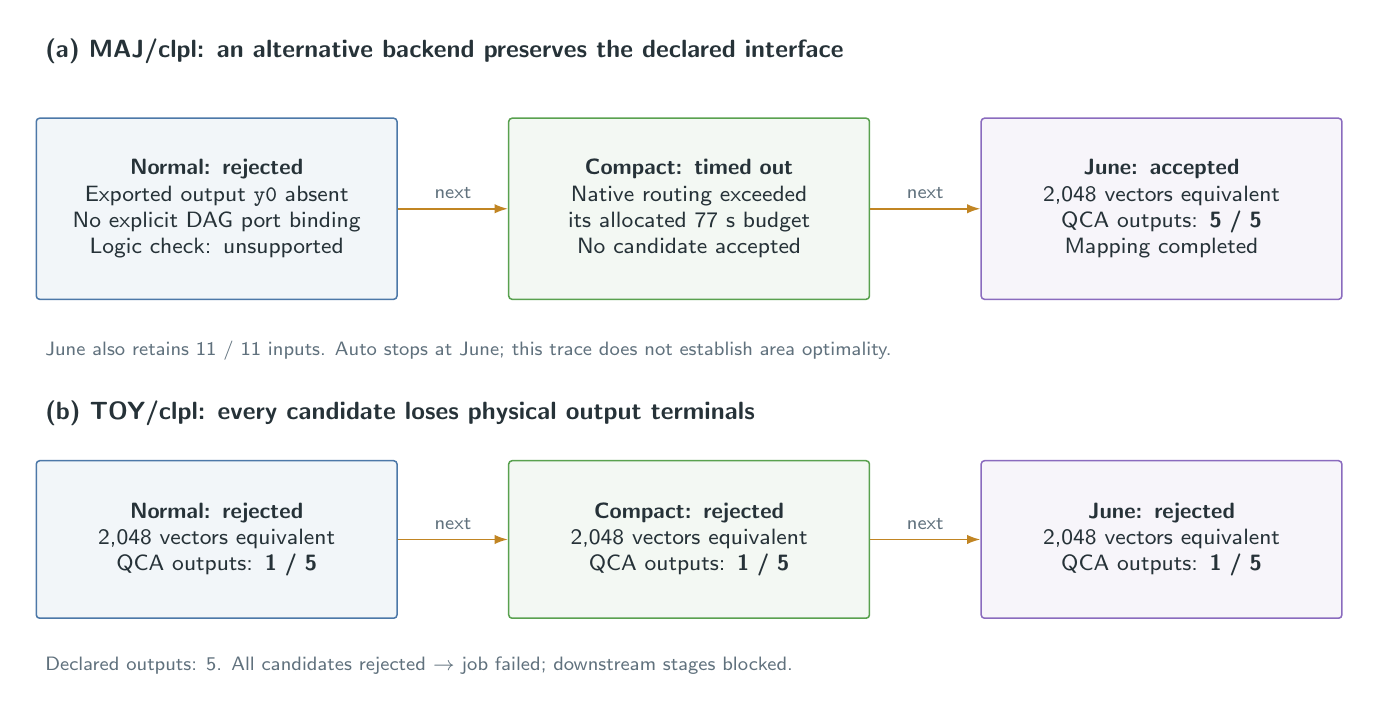
\begin{tikzpicture}[x=1mm,y=1mm]
  \path[use as bounding box] (0,0) rectangle (168,84);
  \node[paneltitle] at (1,81) {(a) MAJ/clpl: an alternative backend preserves the declared interface};
  \node[box,draw=normal,fill=normal!7,text width=43mm,minimum height=23mm] (mn) at (24,61)
    {\textbf{Normal: rejected}\\Exported output \texttt{y0} absent\\No explicit DAG port binding\\Logic check: unsupported};
  \node[box,draw=compact,fill=compact!7,text width=43mm,minimum height=23mm] (mc) at (84,61)
    {\textbf{Compact: timed out}\\Native routing exceeded\\its allocated 77 s budget\\No candidate accepted};
  \node[box,draw=june,fill=june!7,text width=43mm,minimum height=23mm] (mj) at (144,61)
    {\textbf{June: accepted}\\2,048 vectors equivalent\\QCA outputs: \textbf{5 / 5}\\Mapping completed};
  \draw[retry] (mn.east) -- node[smallnote,above] {next} (mc.west);
  \draw[retry] (mc.east) -- node[smallnote,above] {next} (mj.west);
  \node[smallnote,anchor=west] at (1,43)
    {June also retains 11 / 11 inputs. Auto stops at June; this trace does not establish area optimality.};
  \node[paneltitle] at (1,35) {(b) TOY/clpl: every candidate loses physical output terminals};
  \node[box,draw=normal,fill=normal!7,text width=43mm,minimum height=20mm] (tn) at (24,19)
    {\textbf{Normal: rejected}\\2,048 vectors equivalent\\QCA outputs: \textbf{1 / 5}};
  \node[box,draw=compact,fill=compact!7,text width=43mm,minimum height=20mm] (tc) at (84,19)
    {\textbf{Compact: rejected}\\2,048 vectors equivalent\\QCA outputs: \textbf{1 / 5}};
  \node[box,draw=june,fill=june!7,text width=43mm,minimum height=20mm] (tj) at (144,19)
    {\textbf{June: rejected}\\2,048 vectors equivalent\\QCA outputs: \textbf{1 / 5}};
  \draw[retry] (tn.east) -- node[smallnote,above] {next} (tc.west);
  \draw[retry] (tc.east) -- node[smallnote,above] {next} (tj.west);
  \node[smallnote,anchor=west] at (1,3)
    {Declared outputs: 5. All candidates rejected $\rightarrow$ job failed; downstream stages blocked.};
\end{tikzpicture}
\end{document}
